\chapter{Anexos}
\label{cap:anex}


\section{Museu da Pessoa — tratamento de fotografias}
\label{seq:anex-museu}

\subsection{Filtro de Texto}
\label{seq:anex-museu-filtro}
\verbatiminput{anexos/2-1/C/parte_lex.l}

\subsection{Estrutura de dados}
\label{seq:anex-museu-est}
\lstinputlisting[language=c]{anexos/2-1/C/album.c}

\subsection{Cabeçalho ficheiro C}
\label{seq:anex-museu-header}
\lstinputlisting[language=c]{anexos/2-1/C/album.h}

\subsection{Testes}
\label{seq:anex-museu-test}
\subsubsection{Input teste 1}
\label{seq:anex-museu-test-in01}
\lstinputlisting[language=xml,breaklines=true]{anexos/2-1/Exemplo1/legenda.xml}

\subsubsection{Output teste 1}
\label{seq:anex-museu-test-out01-01}
\lstinputlisting[language=html,breaklines=true]{anexos/2-1/Exemplo1/AlbumGerado.html}

\begin{figure}[H]
\centering

\includegraphics[width=15cm]{anexos/2-1/Exemplo1/Screenshots/indice.png}
\caption{Indice HTML gerado pelo ficheiro XML}
\end{figure}

\label{seq:anex-museu-test-out01-02}
\lstinputlisting[language=html,breaklines=true]{anexos/2-1/Exemplo1/1.html}

\begin{figure}[H]
\centering
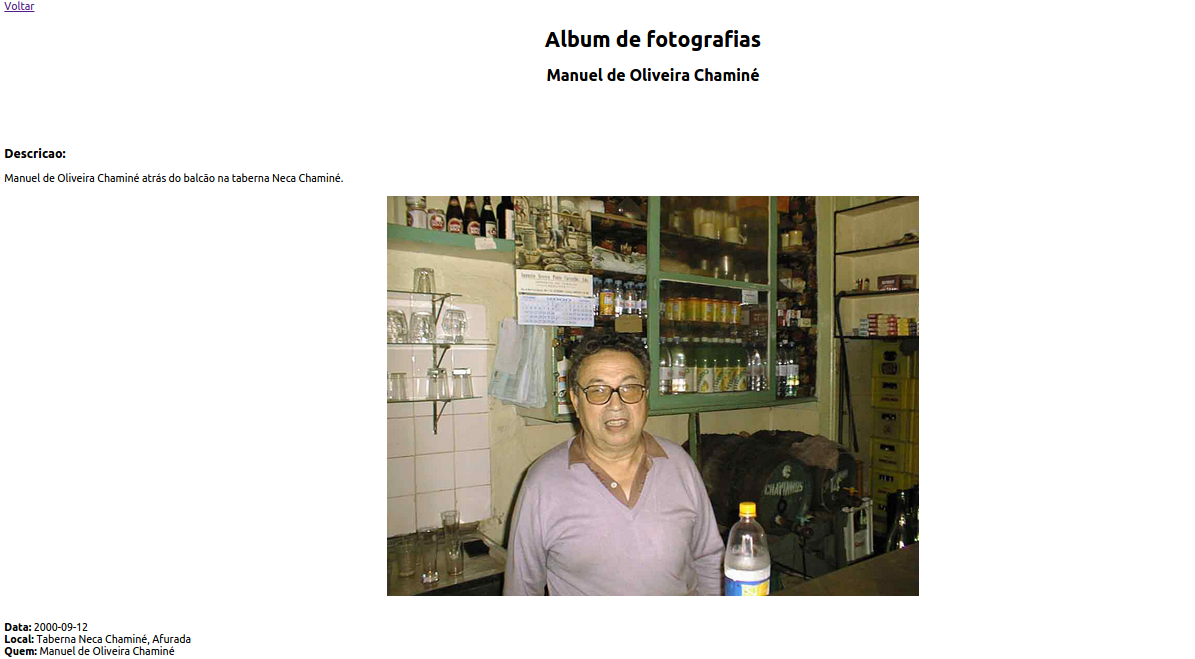
\includegraphics[width=15cm]{anexos/2-1/Exemplo1/Screenshots/pag1.png}
\caption{Pagina HTML gerada pelo ficheiro XML (1 de 2)}
\end{figure}

\begin{figure}[H]
\centering
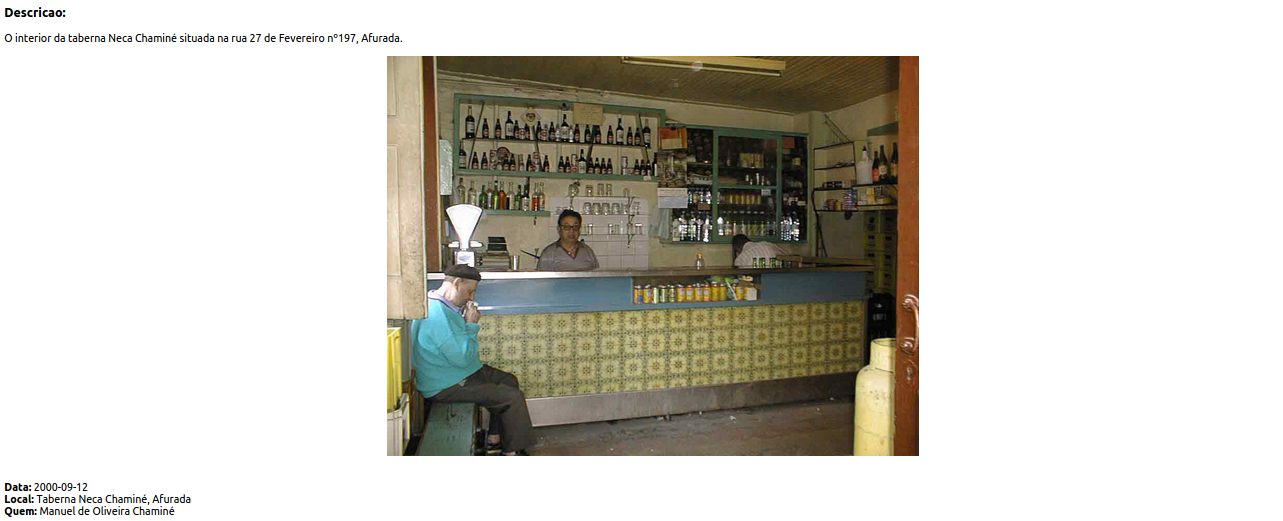
\includegraphics[width=15cm]{anexos/2-1/Exemplo1/Screenshots/pag2.png}
\caption{Pagina HTML gerada pelo ficheiro XML (2 de 2)}
\end{figure}

\subsubsection{Input teste 2}
\label{seq:anex-museu-test-in02}
\lstinputlisting[language=xml,breaklines=true]{anexos/2-1/Exemplo2/legenda.xml}

\subsubsection{Output teste 2}
\label{seq:anex-museu-test-out02-01}
\lstinputlisting[language=html,breaklines=true]{anexos/2-1/Exemplo2/AlbumGerado.html}

\begin{figure}[H]
\centering

\includegraphics[width=15cm]{anexos/2-1/Exemplo2/Screenshots/indice.png}
\caption{Indice HTML gerado pelo ficheiro XML}
\end{figure}

\label{seq:anex-museu-test-out02-02}
\lstinputlisting[language=html,breaklines=true]{anexos/2-1/Exemplo2/5.html}

\begin{figure}[H]
\centering
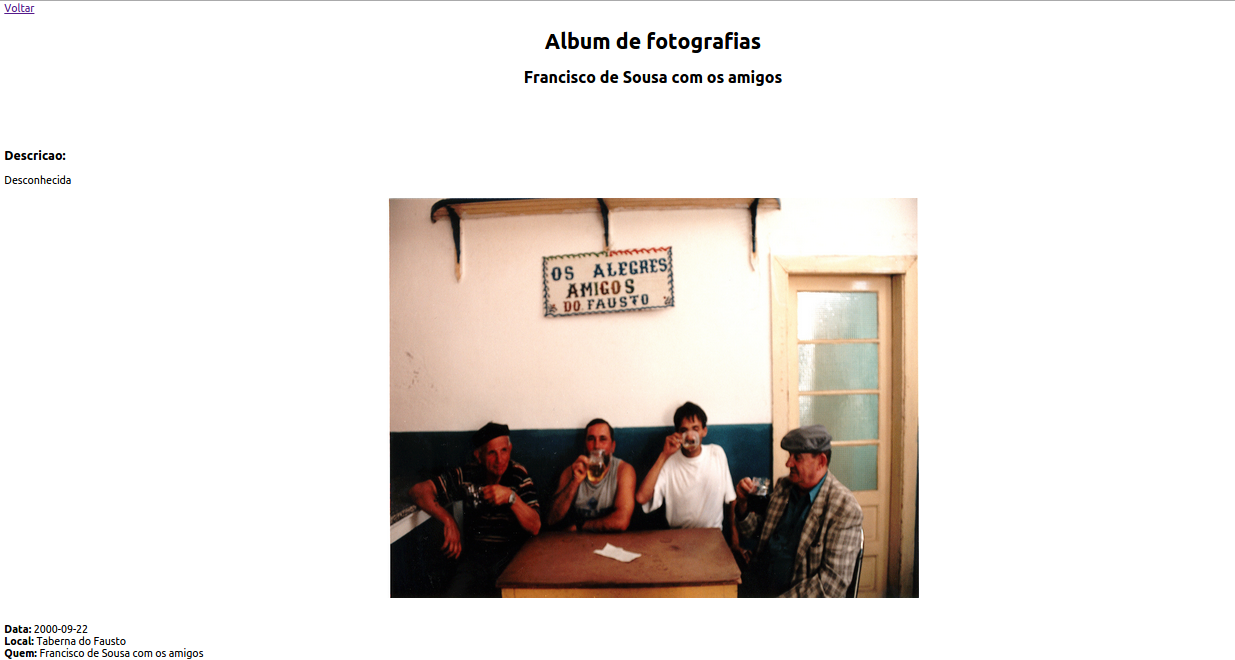
\includegraphics[width=15cm]{anexos/2-1/Exemplo2/Screenshots/pag1.png}
\caption{Pagina HTML gerada pelo ficheiro XML}
\end{figure}

\label{seq:anex-museu-test-out02-03}
\lstinputlisting[language=html,breaklines=true]{anexos/2-1/Exemplo2/6.html}

\begin{figure}[H]
\centering
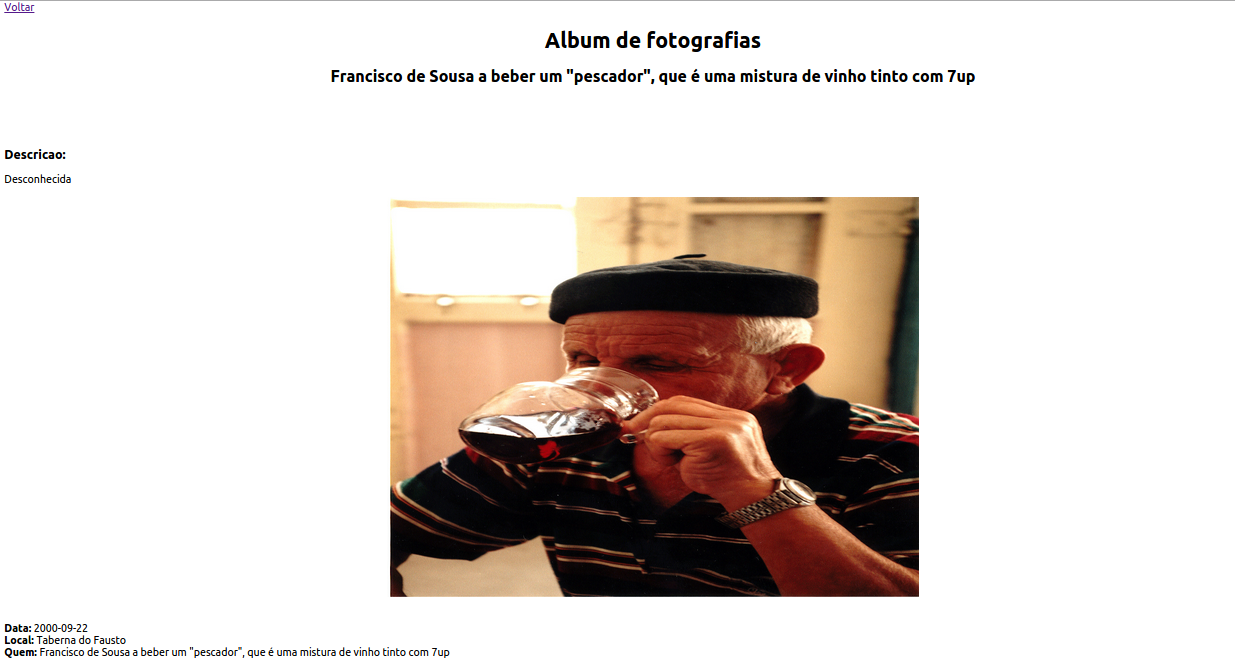
\includegraphics[width=15cm]{anexos/2-1/Exemplo2/Screenshots/pag2.png}
\caption{Pagina HTML gerada pelo ficheiro XML}
\end{figure}

\subsubsection{Input teste 3}
\label{seq:anex-museu-test-in03}
\lstinputlisting[language=xml,breaklines=true]{anexos/2-1/Exemplo3/legenda.xml}

\subsubsection{Output teste 3}
\label{seq:anex-museu-test-out03-01}
\lstinputlisting[language=html,breaklines=true]{anexos/2-1/Exemplo3/AlbumGerado.html}

\begin{figure}[H]
\centering

\includegraphics[width=15cm]{anexos/2-1/Exemplo3/Screenshots/indice.png}
\caption{Indice HTML gerado pelo ficheiro XML}
\end{figure}

\label{seq:anex-museu-test-out03-02}
\lstinputlisting[language=html,breaklines=true]{anexos/2-1/Exemplo3/3.html}

\begin{figure}[H]
\centering
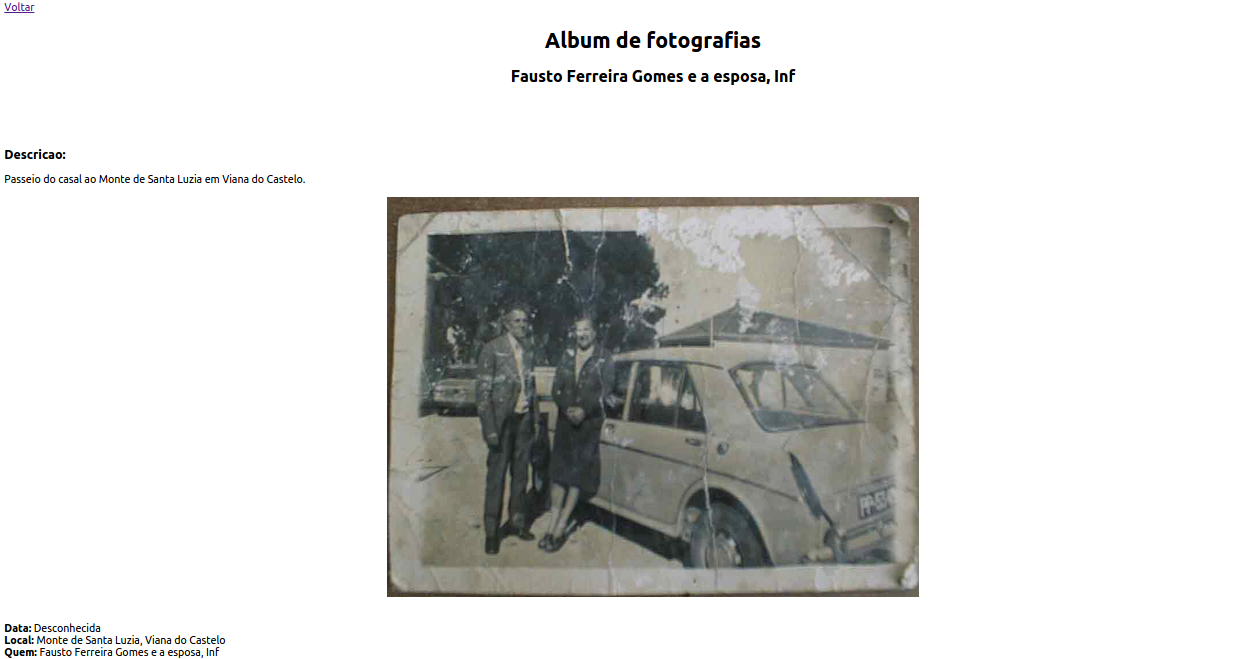
\includegraphics[width=15cm]{anexos/2-1/Exemplo3/Screenshots/pag2.png}
\caption{Pagina HTML gerada pelo ficheiro XML}
\end{figure}

\label{seq:anex-museu-test-out03-03}
\lstinputlisting[language=html,breaklines=true]{anexos/2-1/Exemplo3/4.html}

\begin{figure}[H]
\centering
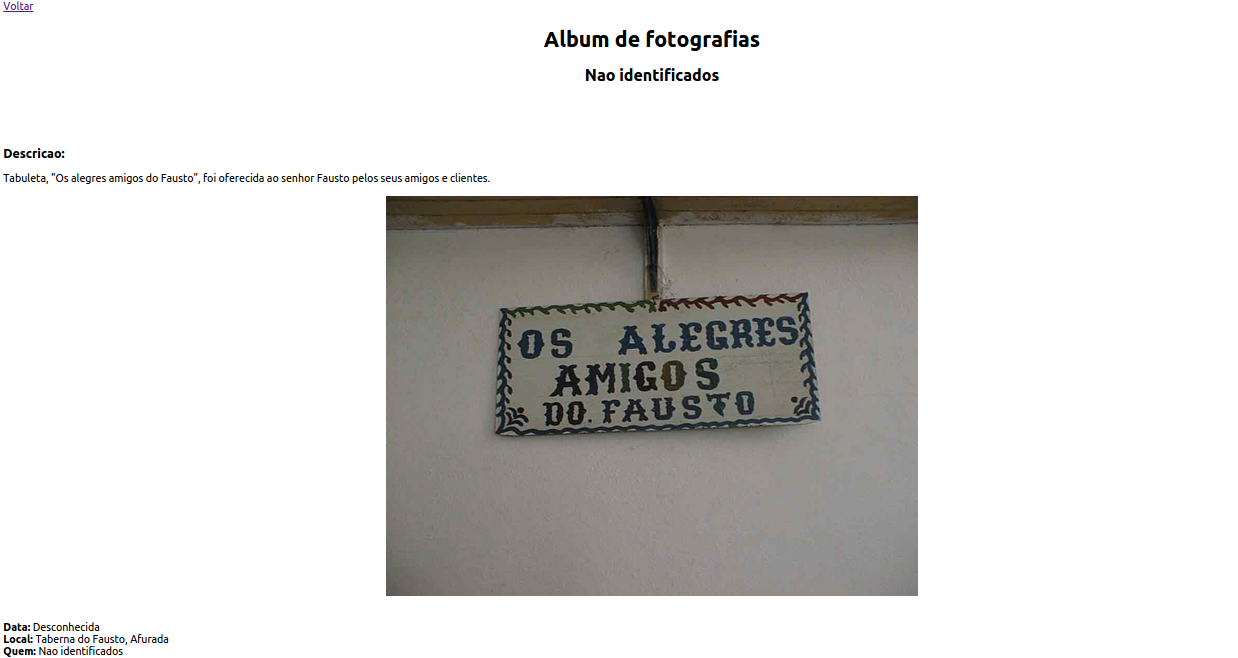
\includegraphics[width=15cm]{anexos/2-1/Exemplo3/Screenshots/pag1.png}
\caption{Pagina HTML gerada pelo ficheiro XML}
\end{figure}

\subsubsection{Input teste 4}
\label{seq:anex-museu-test-in04}
\lstinputlisting[language=xml,breaklines=true]{anexos/2-1/Exemplo4/exemplo.xml}

\subsubsection{Output teste 4}
\label{seq:anex-museu-test-out04-01}
\lstinputlisting[language=html,breaklines=true]{anexos/2-1/Exemplo4/AlbumGerado.html}

\begin{figure}[H]
\centering

\includegraphics[width=15cm]{anexos/2-1/Exemplo4/Screenshots/indice.png}
\caption{Indice HTML gerado pelo ficheiro XML}
\end{figure}

\label{seq:anex-museu-test-out04-02}
\lstinputlisting[language=html,breaklines=true]{anexos/2-1/Exemplo4/1.html}

\begin{figure}[H]
\centering
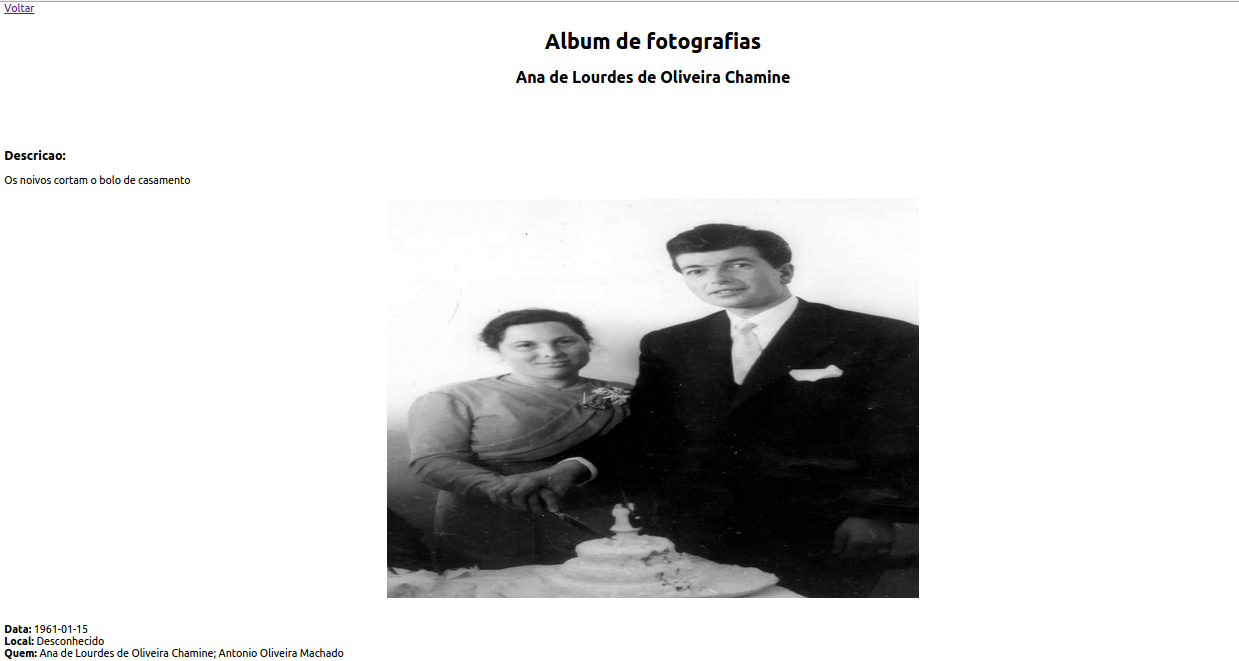
\includegraphics[width=15cm]{anexos/2-1/Exemplo4/Screenshots/pag1.png}
\caption{Pagina HTML gerada pelo ficheiro XML}
\end{figure}

\label{seq:anex-museu-test-out04-03}
\lstinputlisting[language=html,breaklines=true]{anexos/2-1/Exemplo4/2.html}

\begin{figure}[H]
\centering
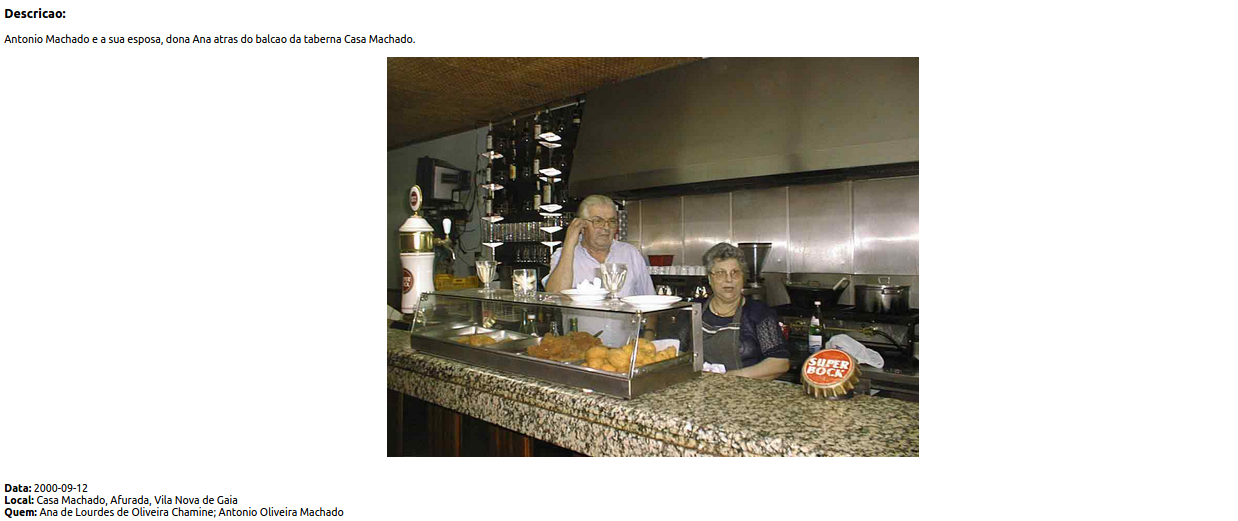
\includegraphics[width=15cm]{anexos/2-1/Exemplo4/Screenshots/pag2_2.png}
\caption{Pagina HTML gerada pelo ficheiro XML}
\end{figure}

\section{Processamento de Entidades Nomeadas (Enamex)}
\label{seq:anex-enamex}

\subsection{Filtro de Texto}
\label{seq:anex-enamex-filtro}
\verbatiminput{anexos/2-2/enamex.l}

\subsection{Estrutura de dados}
\label{seq:anex-enamex-est}
\lstinputlisting[language=c]{anexos/2-2/tree.c}

\subsection{Cabeçalho ficheiro C}
\label{seq:anex-enamex-header}
\lstinputlisting[language=c]{anexos/2-2/tree.h}


\subsection{Testes}
\label{seq:anex-enamex-test}
\subsubsection{Input teste 1}
\label{seq:anex-enamex-test-in01}
\lstinputlisting[language=xml,breaklines=true]{anexos/2-2/teste1_locais.txt}

\subsubsection{Output teste 1}
\label{seq:anex-enamex-test-out01}
\verbatiminput{anexos/2-2/2-5-a-out}
\begin{figure}[H]
\centering
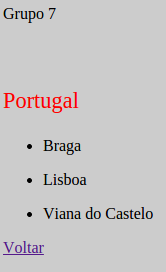
\includegraphics[width=4cm]{anexos/2-2/output_teste1.png}
\end{figure}


\subsubsection{Input teste 2}
\label{seq:anex-enamex-test-in02}
\lstinputlisting[language=xml,breaklines=true]{anexos/2-2/teste2_enunciado.txt}

\subsubsection{Output teste 2}
\label{seq:anex-enamex-test-out02}
\verbatiminput{anexos/2-2/2-5-a-out}
\begin{figure}[H]
\centering
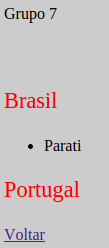
\includegraphics[width=4cm]{anexos/2-2/output_teste2.png}
\end{figure}

\subsubsection{Input teste 3}
\label{seq:anex-enamex-test-in03}
\lstinputlisting[language=xml,breaklines=true]{anexos/2-2/teste3_internet.txt}

\subsubsection{Output teste 3}
\label{seq:anex-enamex-test-out03}
\verbatiminput{anexos/2-2/2-5-a-out}
\begin{figure}[H]
\centering
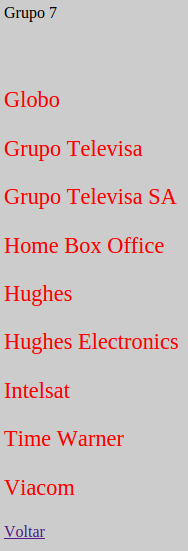
\includegraphics[width=4cm]{anexos/2-2/output_teste3.png}
\end{figure}






\section{Processamento de ficheiros com Canções}
\label{seq:anex-music}

\subsection{Filtro de Texto}
\label{seq:anex-music-filtro}
\verbatiminput{anexos/2-5/flex.l}

\subsection{Estrutura de dados}
\label{seq:anex-music-est}
\lstinputlisting[language=c]{anexos/2-5/musica.c}

\subsection{Cabeçalho ficheiro C}
\label{seq:anex-music-header}
\lstinputlisting[language=c]{anexos/2-5/musica.h}

\subsection{Testes}
\label{seq:anex-music-tests}
\subsubsection{Input teste 1}
\label{seq:anex-music-test-in01}
\verbatiminput{anexos/2-5/2-5-a-in}

\subsubsection{Output teste 1}
\label{seq:anex-music-test-out01}
\verbatiminput{anexos/2-5/2-5-a-out}

\subsubsection{Input teste 2}
\label{seq:anex-music-test-in02}
\verbatiminput{anexos/2-5/2-5-a-in}

\subsubsection{Output teste 2}
\label{seq:anex-music-test-out02}
\verbatiminput{anexos/2-5/2-5-b-out}

\subsubsection{Input teste 3}
\label{seq:anex-music-test-in03}
\verbatiminput{anexos/2-5/2-5-c-in}

\subsubsection{Output teste 3}
\label{seq:anex-music-test-out03}
\verbatiminput{anexos/2-5/2-5-c-out}

\begin{figure}
\centering
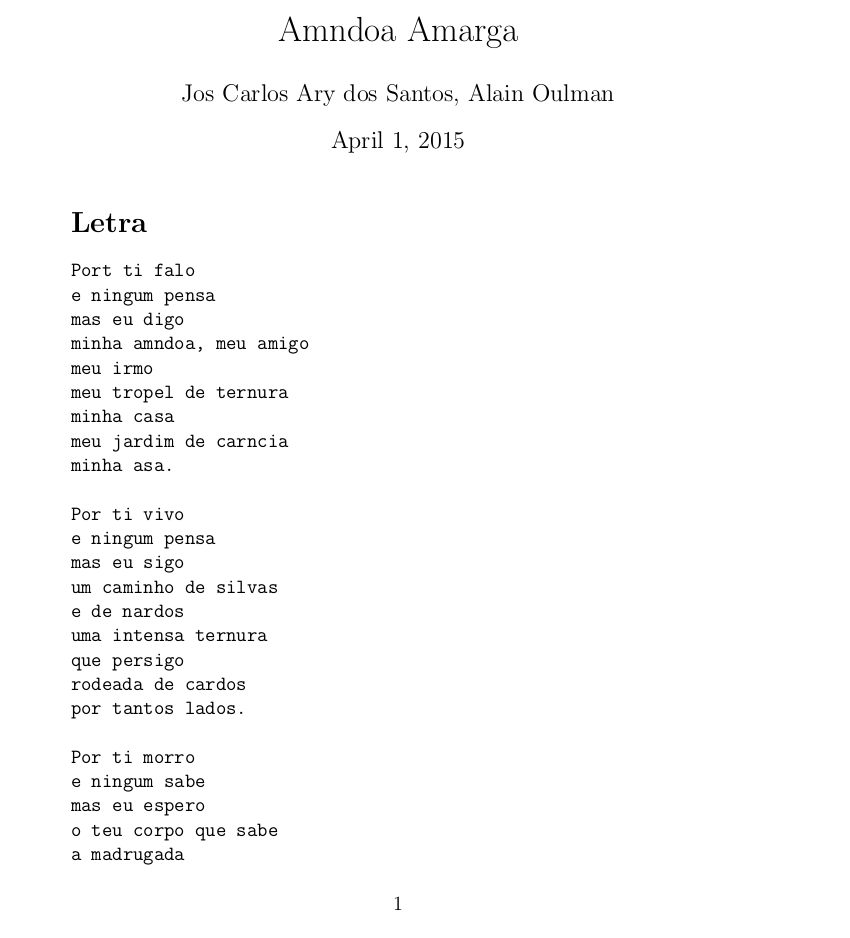
\includegraphics[width=15cm]{anexos/2-5/2-5-a-img1.png}
\caption{PDF gerado por o ficheiro latex (teste 1). Pagina 1 de 2}
\end{figure}

\begin{figure}
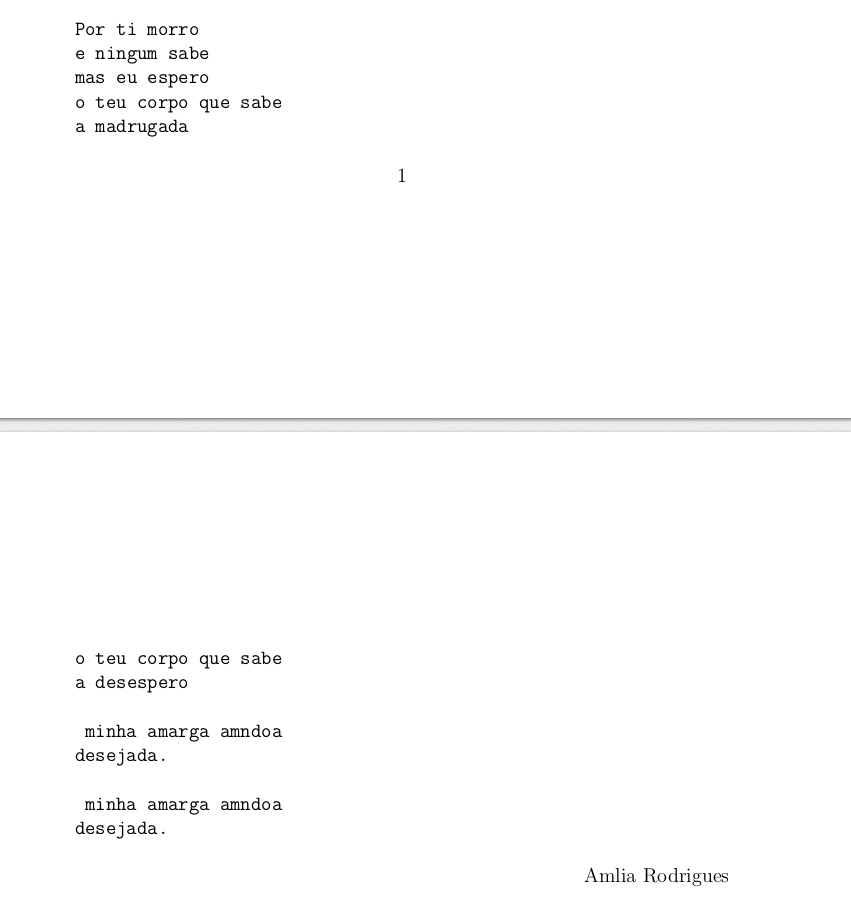
\includegraphics[width=15cm]{anexos/2-5/2-5-a-img2.png}
\caption{PDF gerado por o ficheiro latex (teste 1). Pagina 2 de 2}
\label{fig::anex-music-test-img}
\end{figure}

\begin{figure}
\centering
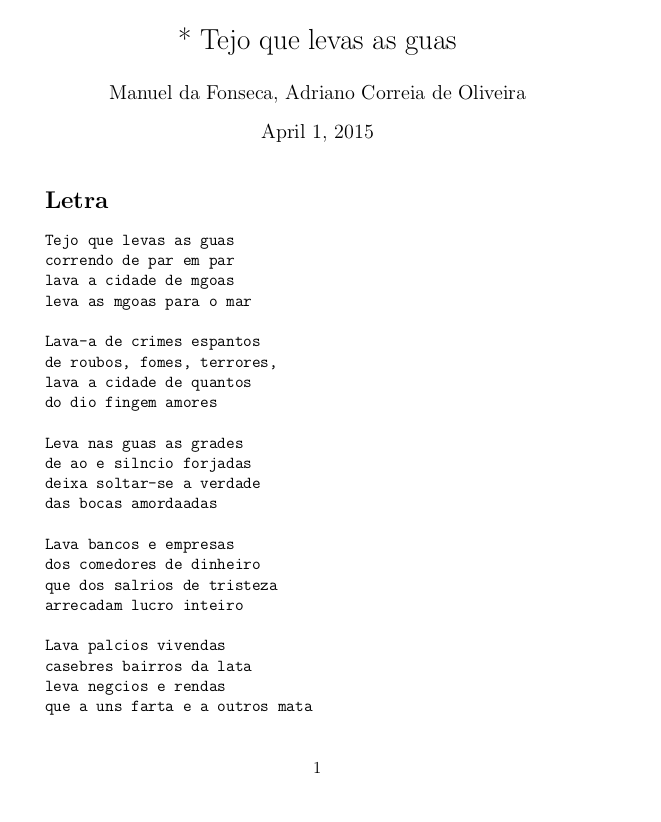
\includegraphics[width=15cm]{anexos/2-5/2-5-b-img.png}
\caption{PDF gerado por o ficheiro latex (teste 2). Pagina 1 de 2}
\label{fig::anex-music-test-img02}
\end{figure}

\begin{figure}
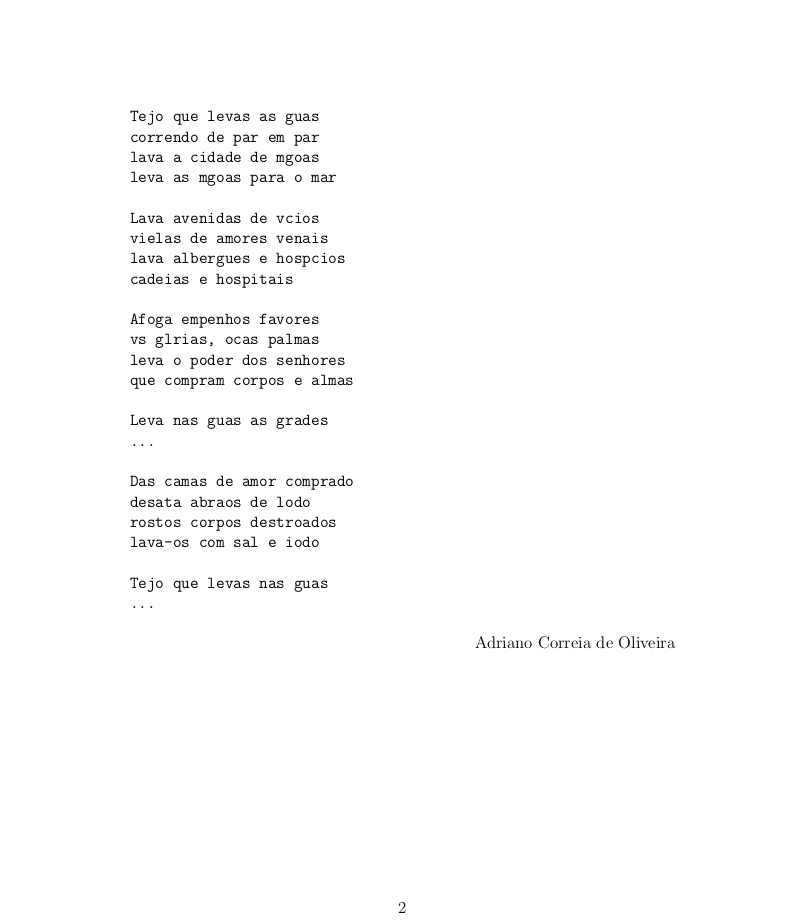
\includegraphics[width=15cm]{anexos/2-5/2-5-b-img2.png}
\caption{PDF gerado por o ficheiro latex (teste 2). Pagina 2 de 2}
\label{fig::anex-music-test-img}
\end{figure}

\begin{figure}
\centering
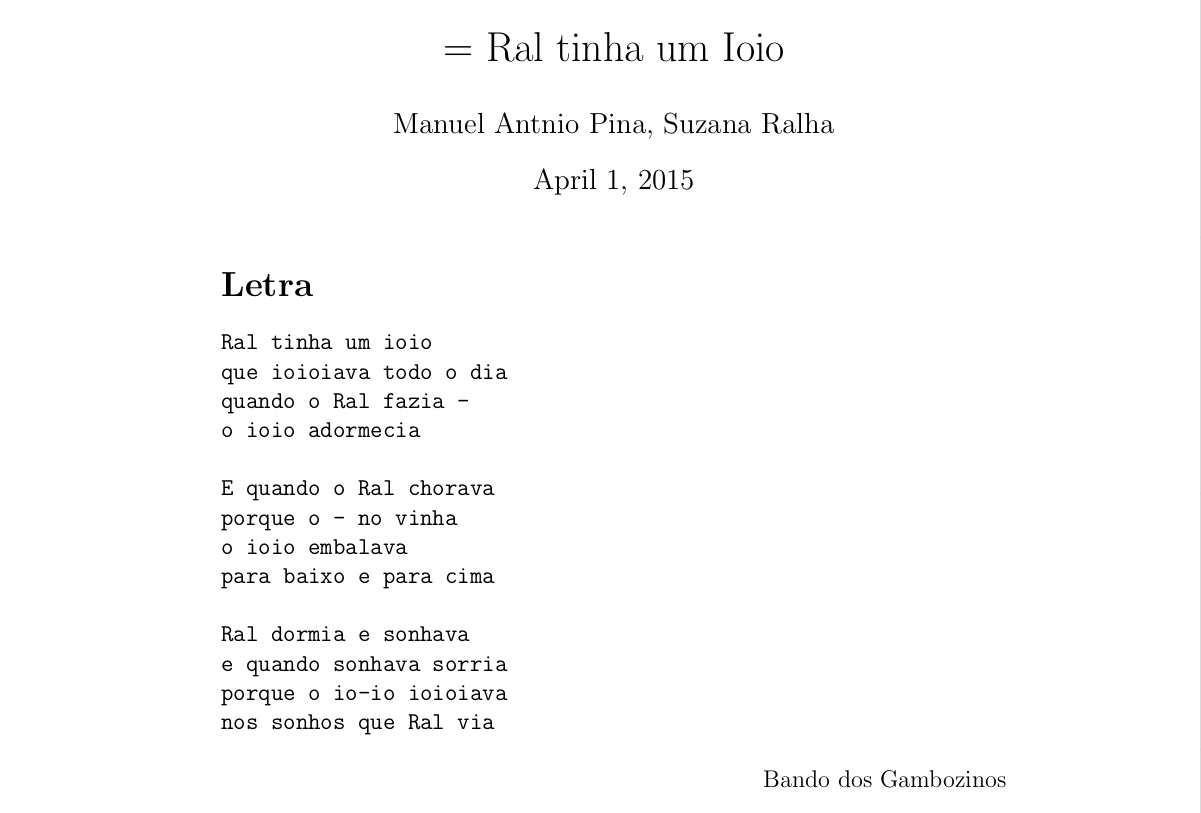
\includegraphics[width=15cm]{anexos/2-5/2-5-c-img.png}
\caption{PDF gerado por o ficheiro latex (teste 3)}
\label{fig::anex-music-test-img03}
\end{figure}